\chapter{State of the Art} \label{sec:cap2}

\section{Introduction to Nuclear Fusion}

Nuclear fusion is the process in which two light atomic nuclei combine to form a heavier nucleus, releasing a substantial amount of energy. This is the same reaction that powers the Sun and other stars, making it a potential source of clean, virtually limitless energy for humanity.

The primary fuels for fusion are hydrogen isotopes such as deuterium and tritium. Their fusion produces helium and a high-energy neutron, releasing energy mainly as the kinetic energy of the neutron and, to a lesser extent, electromagnetic radiation.

Achieving controlled fusion on Earth requires overcoming the electrostatic repulsion between positively charged nuclei, which demands extremely high temperatures (on the order of tens of millions of kelvin) and sufficient pressure. These conditions can be achieved through magnetic confinement — in devices known as tokamaks — or through inertial confinement using high-power lasers.


\section{Nuclear Fusion on \acs{ITER} and \acs{JET}}

The \ac{ITER} project is an international collaboration aimed at demonstrating the feasibility of nuclear fusion  project is an international collaboration designed to demonstrate the feasibility of nuclear fusion as a large-scale, carbon-free energy source. Under construction in Cadarache, France, ITER involves 35 countries, including members of the European Union, the United States, China, India, Japan, Russia, and South Korea. It will house the world's largest tokamak, using magnetic confinement to heat plasma to fusion conditions.\ \ac{ITER} is designed to produce ten times more fusion power than the power used to heat the plasma, representing a major step toward commercial fusion energy.

The \ac{JET} tokamak, located in the United Kingdom, is currently the largest operational tokamak and has played a key role in advancing fusion science. \ac{JET} has been essential for testing plasma scenarios, materials, and technologies that will be implemented in \ac{ITER}, achieving record plasma parameters and significant advances in stability and confinement.

The \ac{CIEMAT} is Spain's representative in \ac{EURATOM}'s fusion program, which includes participation in \ac{JET} and \ac{ITER}. For this project, \ac{CIEMAT} has provided experimental data from \ac{JET}, consisting of recorded plasma discharges.

\section{Discharges and Disruptions}

A \textit{Discharge} is a plasma operation in the tokamak, where the plasma is created and maintained for a certain period. Each discharge is characterized by various parameters, such as plasma current, inductance, density, radiated power or input power. When these parameters deviate from their expected values, it can indicate potential issues or anomalies in the reactor's operation.

A \textit{Disruption} is an event that occurs when the plasma becomes unstable and loses confinement, leading to a rapid cooling of the plasma and a loss of control. For this project, discharges are classified as either disruptive or non-disruptive.

A \textit{Campaign} is a set of discharges that are analyzed together. For this project, there are three campaigns available, each containing a different number of discharges. The available data for the project is summarized in \autoref{tab:campaigns}. This data is collected from the \ac{JET} tokamak and stored in text files for later analysis.

\begin{table}[htbp]
    \centering
    \caption{Available data for the project}
    \begin{tabular}{
        l
        S[table-format=3]  % Number of discharges
        S[table-format=2]  % Disruptive
        S[table-format=3]  % Non Disruptive
        S[table-format=1.2]@{\,}  % Rate
    }
    \toprule
    \textbf{Campaign} & \textbf{Discharges} & \textbf{Disruptive} & \textbf{Non--Disruptive} & \textbf{Disruptive Rate} \\
    \midrule
    C23 & 522 & 32 & 490 & 6.13 \ \% \\
    C24 & 388 & 26 & 362 & 6.70 \ \% \\
    C25 & 611 & 41 & 570 & 6.71 \ \% \\
    \bottomrule
    \end{tabular}
    \label{tab:campaigns}
\end{table}

A visual representation of the plasma current on several discharges is shown in \autoref{fig:plasma-current}. This figure illustrates the singular bathtub shape of non-disruptive discharges, whereas disruptive discharges show a more erratic pattern.

\begin{figure}[H]
    \centering
    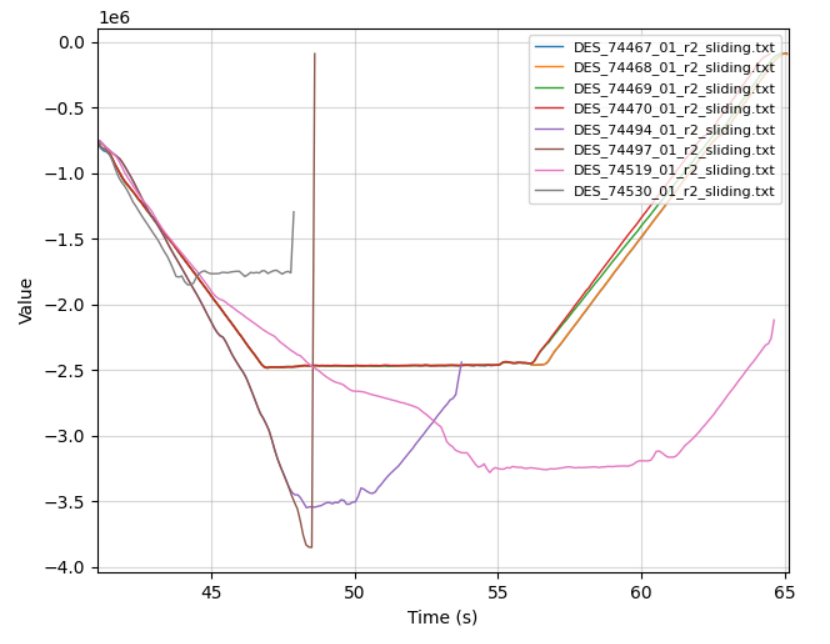
\includegraphics[width=0.8\textwidth]{plasma-current.png}
    \caption{Plasma current on disruptive and non-disruptive discharges}
    \label{fig:plasma-current}
\end{figure}

\section{Anomaly Detection in Nuclear Fusion}

Anomaly detection in nuclear fusion is crucial for ensuring the safe and efficient operation of reactors like \ac{ITER}. The complexity of the plasma behavior and the multitude of parameters involved make it challenging to monitor and control the system effectively. Anomalies can lead to disruptions, which can damage the reactor components and affect the overall performance.

To address this challenge, various machine learning techniques have been applied to analyze the data generated during discharges. These techniques aim to identify patterns and deviations in the data that may indicate potential anomalies. An early detection of these anomalies is essential to prevent disruptions and ensure the stability of the plasma, using gas injection to stop the nuclear fusion reaction before it causes damage to the reactor.

\subsection{Introduction to \acs{APODIS}}

\ac{CIEMAT} uses the \ac{APODIS} algorithm, which is based on a \ac{SVM} model trained on historical discharge data. The model is designed to classify discharges as normal or anomalous based on the input parameters. The training process involves using labeled data, where each discharge is categorized as either normal or anomalous.

The \ac{APODIS} algorithm uses the signals listed in \autoref{tab:apodis-signals}.

\begin{table}[htbp]
  \centering
  \caption{List of signals analysed in the APODIS algorithm}
  \label{tab:apodis-signals}
  \begin{tabular}{@{}l c@{}}
    \toprule
    \textbf{Signal Name} & \textbf{Units} \\
    \midrule
    (1) Plasma Current                             & \si{A} \ \ \  \\
    (2) Mode Lock Amplitude                        & \si{T} \ \ \  \\
    (3) Plasma internal inductance                 &             \\ % adimensional
    (4) Plasma density                             & \si{\per\cubic\metre} \\
    (5) Stored diamagnetic energy time derivative  & \si{W} \ \ \  \\
    (6) Radiated Power                             & \si{W} \ \ \  \\
    (7) Total Input power                          & \si{W} \ \ \  \\
    \bottomrule
  \end{tabular}
\end{table}

\section{Machine Learning}
\ac{SVM} is a machine learning algorithm whose goal is to find the optimal hyperplane that separates the data into different classes \autocite{6524743}. On the training phase, the model receives entire discharges as input, and the category of the discharge. Then, it divides data in windows of 32 milliseconds, and extracts the mean value and the \ac{FFT} of each window. On the prediction phase, the model receives a data stream, and fills a buffer to create a window. Then, it extracts the same features as in the training phase, and predicts the category of this window. If the model predicts an anomalous window, the discharge is classified as anomalous. This classification shall be done before the disruption occurs.

There are some limitations to this approach. First, a window-based approach does not take into account the temporal dependencies of the data. This means that the model may not be able to capture the dynamics of the plasma behavior over time. Second, \ac{SVM} models with non-linear kernels have a complexity between $O(n^2)$ and $O(n^3)$, where $n$ is the number of training samples. This means that the model may not be able to scale to large datasets \autocite{kekulawalaSupportVectorMachines2024}. Third, even though \ac{SVM} models do not require a balanced dataset, the model could be biased towards the majority class, leading to a high false negative rate \autocite{10.1007/978-3-540-30115-8_7}. This is particularly important in this project, as the number of non-disruptive discharges is much higher than the number of disruptive discharges, as shown in \autoref{tab:campaigns}.

\section{Alternative approaches}

This project aims to explore alternative approaches to anomaly detection in nuclear fusion, focusing on the use of other \ac{ML} algorithms. Models used in this project can be grouped into three categories: decision trees based models, machine vector support based models and deep learning models. For each category, there are two subcategories: outlier detection and binary classification. Outlier detection models are trained on a single class of data (non-disruptive discharges), and generate a decision boundary that separates the normal data from the anomalies. Supervised binary classification models are trained on both classes of data (disruptive and non-disruptive discharges), and generate a decision boundary that separates the two classes.

\subsection{Decision Trees based models}

Decision trees are a type of \ac{ML} algorithm that uses a tree-like structure to make decisions based on the input data. This structure is built at the training phase, where the algorithm recursively splits the data into subsets based on the features that provide the most information gain. The resulting tree can be used to classify new data points by following the branches of the tree based on their feature values \autocite{1522531}.

\subsubsection{Outlier detection}

Decision trees can be used for outlier detection by training the model on a single class of data (non-disruptive discharges) and identifying instances that fall outside the normal patterns. The decision tree learns the characteristics of the normal data and can flag instances that do not conform to these patterns as potential anomalies. 

\ac{IForest} is the canonical example of this approach. It splits the data at random features and thresholds, creating a forest of trees. Anomalies tend to be isolated in fewer splits than normal instances, because they lie in sparse regions of the feature space \autocite{inproceedings}. Later improvements, like Extended Isolation Forest replace axis-aligned cuts with random hyperplanes to reduce bias \autocite{haririExtendedIsolationForest2019}.

\subsubsection{Binary classification}

If labelled data of both classes exist, standard decision-tree classifiers or ensembles (Random Forests, Gradient Boosting) can draw an explicit boundary between them. With sufficient minority class samples, these models usually outperform outlier detection models, as the tree learns exactly which feature ranges characterize each class rather than inferring a boundary from a single class. In practice, binary trees are common in fraud detection and network-intrusion datasets, where even a modest number of confirmed attack records allows the model to reach high recall without over-flagging harmless traffic \autocite{354051491,binary-classification-for-fraud-detection}.

For this project, a \ac{GBDT} classifier with a logistic objective is employed. The ensemble produces an additive margin
\[
F(x)=\sum_{t=1}^{T} f_t(x),
\]
which is mapped to a sigmoidal score
\begin{equation}
p(x)=\sigma\big(F(x)\big)=\frac{1}{1+e^{-F(x)}}.
\label{eq:gbdt-sigmoid}
\end{equation}
The regularized training objective is
\begin{equation}
\mathcal{L}(\{f_t\}) \;=\; \sum_{i=1}^{N} w_i\,\ell\!\left(y_i,\,F(x_i)\right) \;+\; \sum_{t=1}^{T} \Omega\!\left(f_t\right),
\label{eq:gbdt-objective}
\end{equation}
where \(y_i\in\{0,1\}\) are labels, \(w_i>0\) are sample or class weights, \(\Omega(\cdot)\) penalizes tree complexity (e.g., number of leaves and \(L_2\) regularization of leaf values), and \(\ell\) is the logistic loss

\begin{equation}
\ell(y,F) \;=\; -\,y\,\log \sigma(F)\;-\;(1-y)\,\log\bigl(1-\sigma(F)\bigr).
\label{eq:logistic-loss}
\end{equation}

At each boosting iteration the new tree \(f_t\) is fitted to (an approximation of) the negative gradient of the loss with respect to \(F\), typically using a second-order Taylor expansion to score candidate splits.

The model outputs \(p(x)\in[0,1]\), a monotone transformation of the margin \(F(x)\). Under class or sample reweighting (\(w_i\neq 1\)), \(p(x)\) should be interpreted as a sigmoidal score rather than a calibrated posterior probability; the operating point is therefore chosen on a held-out temporal validation set by selecting a decision threshold \(\tau\) for \(\hat{y}(x)=\mathbb{1}[p(x)\ge\tau]\) that optimizes the task metric \autocite{friedmanGreedyFunctionApproximation2000,chenXGBoostScalableTree2016}.


\subsection{Machine Vector Support based models}

\ac{SVM} is a well-known algorithm in this category, but there are other algorithms that can be used as well. For example, \ac{OC-SVM} is a variant of \ac{SVM} that is trained on a single class of data (non-disruptive discharges), and generates a decision boundary that separates the normal data from the anomalies. This approach is particularly useful when the dataset highly imbalanced.

\todo{SVM, OC-SVM}

\subsection{Deep learning models}
% LSTM & CNN

\todo{LSTM, CNN, Autoencoders}
